\documentclass[a4paper, 12pt]{report}

\usepackage{lmodern}
\usepackage[english]{babel}

\usepackage[left=25mm, bottom=25mm, top=30mm]{geometry}

\usepackage{blindtext}

\usepackage{fancyhdr}
\fancyhf{}
\fancyhead[L]{Machine Learning Project Competition (MLPC) 2022}
\fancyhead[R]{April 2022}
\fancyfoot[L]{Abapathi, Fish Vs Plastic Classifier For Ocean Cleanup}
\fancyfoot[R]{\thepage}
\pagestyle{fancy}

\renewcommand{\thesection}{\arabic{section}}

%For subsubsection to be handled
\setcounter{tocdepth}{3}
\setcounter{secnumdepth}{3}

\usepackage{indentfirst}
\usepackage{url}
\def\UrlBreaks{\do\/\do-}
\usepackage{hyperref}

\usepackage{graphicx}

\begin{document}


\hspace{50mm}
\hspace{50mm}


{\centering\Large\bfseries Abapathi\\ Fish vs plastic classifier for ocean cleanup \par}

\hspace{50mm}
\hspace{50mm}
\hspace{50mm}

\textbf{\flushleft\large Author 1 \hfill AUTHOR1@POLYTECHNIQUE.CM}
{\itshape \\ Computer Science Department\\ National Advanced School of Engineering of Yaounde\\
Yaounde, Cameroon\\
P.O. Box 8390 Yaounde}

\textbf{\flushleft\large Author 2 \hfill AUTHOR2@POLYTECHNIQUE.CM}
{\itshape \\ Computer Science Department\\ National Advanced School of Engineering of Yaounde\\
Yaounde, Cameroon\\
P.O. Box 8390 Yaounde}

\hspace{50mm}
\hspace{50mm}
\hspace{50mm}


\section{Introduction}

Plastic pollution is pollution caused by the accumulation of plastic waste in the environment.The global system of production, use and disposal of plastics is a broken system. Plastic pollution is correlated with the low cost of plastic, which leads to its massive and disposable use. It is also due to the low degradability of plastics. This pollution can have detrimental effects on land, seas and oceans, and waterways by affecting wildlife, habitat and secondarily or through feedback from humans. It is estimated that 24 to 35 million tons of plastic waste enter the aquatic environment each year. Living organisms, particularly marine animals, can be impacted, either through mechanical effects such as entanglement in plastic objects and problems associated with ingestion of plastic waste, or through exposure to chemicals in plastics that interfere with their physiology. Effects on humans include disruption of various hormonal mechanisms. The pollution of the oceans by plastics is therefore a serious problem to which a solution must be found.

In this paper we will build a fish vs plastic classifier that will be able to distinguish between fish images and plastics images, these images being taken in ocean waters. A robot equipped with such a model would be able to scour the depths of ocean waters and retrieve plastic waste without endangering marine animals. 

\section{Related work}

Regarding the problem of cleaning the oceans, at this time the automatic solutions proposed are robots that scour the surface of the water to recover floating plastic waste. The best of them are equipped with an Artificial Intelligence allowing them to detect objects, which allows a more optimal movement on the surface of the water, like the one proposed by Razer \cite{razer_bot}. 

The limit of this solution is that it can only recover the plastics present on the surface, but some of this waste remains at depth, and represents a real danger for marine animals, and consequently for humans. For a robot to be able to carry out this cleaning in deep waters, it would have to be equipped with a program allowing it to recognize and distinguish plastic waste from marine animals. 

Concerning what has already been done, on the one hand a fish detection algorithm has been published by Yu Zhou and Alt \cite{fish_detection}. On the other hand, Gautam Tata proposed an algorithm for the detection of marine plastics, realized with YOLO, and this one having an accuracy of 85\% \cite{plastic_detection}. 

The model we propose will be able to distinguish between fish and plastics with a very good accuracy so that the robot in charge of cleaning will make as few mistakes as possible.

\section{Methodology and implementation}

To successfully achieve this project, we followed a methodology based on four (06) main stages:

\begin{itemize}

    \item The definition and understanding of the problem

    \item Data collection
    
    \item Data preprocessing

    \item Building Deep Learning algorithm using convultional neural network

    \item Training and testing

    \item Result
    
\end{itemize}

\begin{center}

    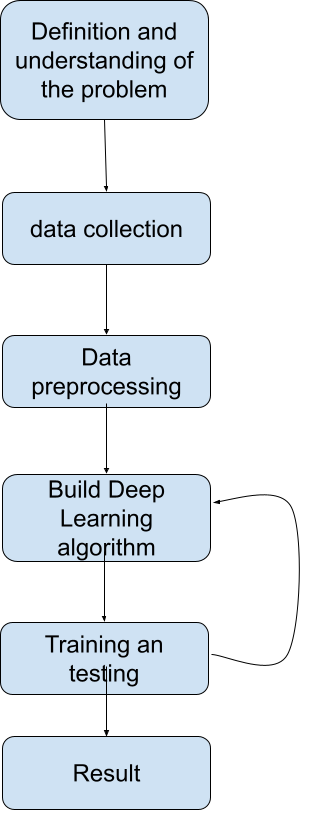
\includegraphics[height = 0.55 \linewidth]{graph.png}

    \textbf{Figure 1: Methodology process}

\end{center}


\subsection{Definition an understanding of the problem}

Most African coastal countries open to the ocean such as Senegal, Ghana, South Africa, Kenya and Cameroon are facing the problem of ocean water pollution. According to UNEP\cite{UNEP}, every year humans produce 300 million tons of plastic garbage, and 11 million of them end up in the oceans. end up in the oceans. Without rapid action on a large scale, these volumes triple by 2040. The plastic never really disappears. It turns into fine particles, which are swallowed by fish or farm animals and eventually consumed by humans through their food and tap water. This leads to an increased risk of cancer and hormonal problems.

As some consequences of pollution of oceans by plastics in the african context we can list :

\begin{itemize}

    \item The ocean provides the primary source of protein for more than one billion people. The threat of marine wildlife poses a danger to the food supply of these populations.

    \item Pollution threatens the job security of workers in the artisanal fishing sector. 

    \item A country like Senegal has as its main source of income the fishing industry.

    \item Strangulation of marine animals.

    \item Waste that has not sunk or been washed ashore, drifts and drift and wash up on our beaches. In addition to constituting a major ecological challenge, they are a visual pollution with real impacts on the local economy. It is thus all the tourist activity that can suffer the consequences: a decrease in the number of tourists, negative image of the town, etc.

\end{itemize}

Following these observations, it is trivial that the pollution of ocean waters is an urgent problem that must be addressed.

\subsection{Data collection}

Data collection is one of the first and most important tasks of a Machine Learning project, since the algorithm will process this data to provide results. The quality of the data used in the construction of the model therefore has a great impact on the quality of the results obtained.

To build our fish vs plastic classifier, we needed as input fish an plastic images taken inside ocean waters. We built our dataset by collecting images from several sources:

\begin{itemize}
    
    \item Almost 10\% of both type of images (fish and plastic) has been selected manually on google, pixabay, unsplash.

    \item 55\% of fish has been taken into the dataset “Fish Species Image Data” on Kaggle\cite{kaggle_fish_1} and 40\% from the dataset “Blue Bot Dataset: Parrot fish”\cite{kaggle_fish_2}.

    \item 95\% of plastic images is from the drive “DeepPlastic”\cite{drive_plastic}.

\end{itemize}

This allowed us to have a balanced dataset of 3550 fish images, and 3600 plastic images.

\subsection{Data preprocessing}

Tensorflow allows to label data automatically.  For our project, we have two classes: a plastic class and a fish class. To label our images, we simply created two folders with the exact names of our classes ("fish" and "plastic") and in each of these folders we respectively put the corresponding images. When loading the images, tensorflow automatically assigns to each image as a class the name of the folder that contains it, and it is also possible to indicate the proportion that will be used for training and for testing.

Below we have some examples of the dataset images.

\begin{center}

    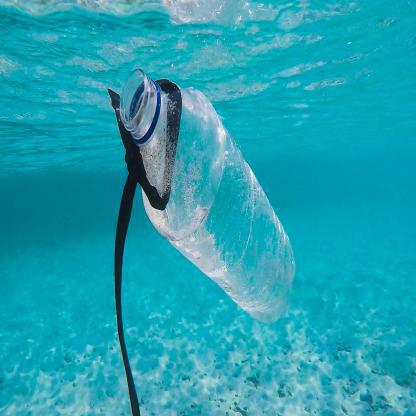
\includegraphics[height = 0.3 \linewidth]{plastic_1.jpg}
    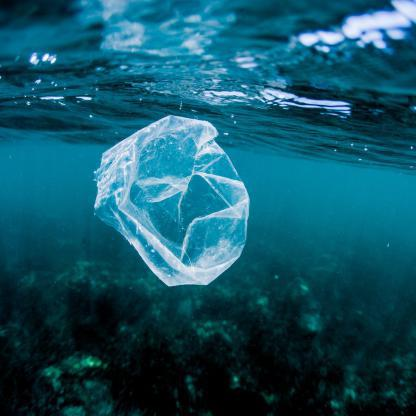
\includegraphics[height = 0.3 \linewidth]{plastic_2.jpg}
    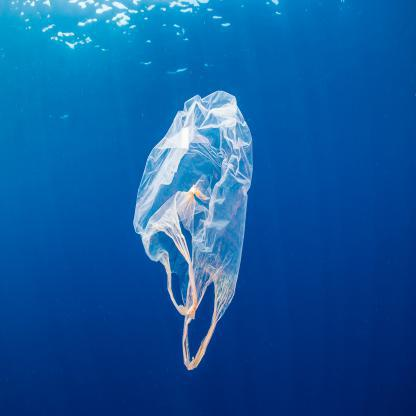
\includegraphics[height = 0.3 \linewidth]{plastic_3.jpg}

    \textbf{Figure 2: examples of plastic images}

\end{center}

\begin{center}

    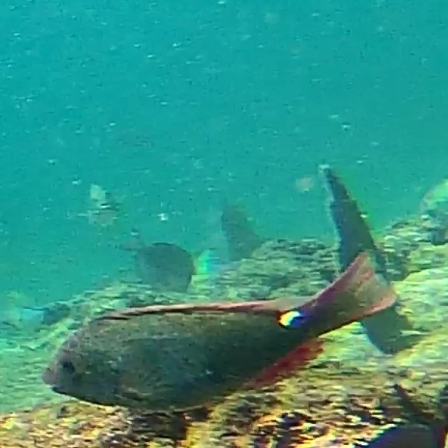
\includegraphics[height = 0.3 \linewidth]{fish_1.jpg}
    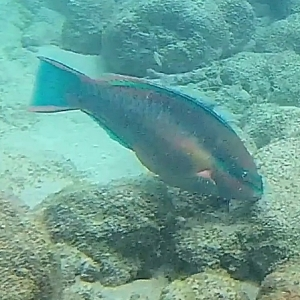
\includegraphics[height = 0.3 \linewidth]{fish_2.jpg}
    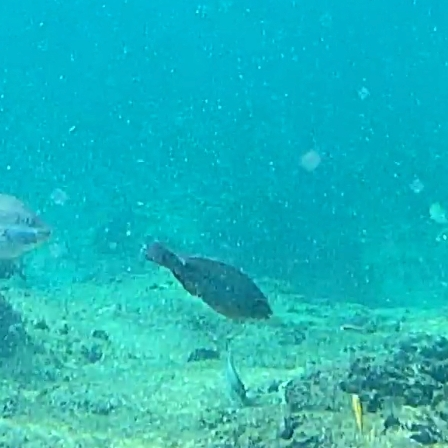
\includegraphics[height = 0.3 \linewidth]{fish_3.jpg}

    \textbf{Figure 3: examples of fish images}

\end{center}

\subsection{Building Deep Learning algorithm}

The problem we are trying to solve falls into the category of image processing. We have therefore chosen to use neural networks to solve it, and more precisely Convolutional Neural Networks (CNN).

The name "convolutional neural network" indicates that the network employs a mathematical operation called convolution. In mathematics convolution is a mathematical operation on two functions that produces a third function that expresses how the shape of one is modified by the other.This kind of neural network uses convolution in place of general matrix multiplication in at least one of their layers. Their architecture involves several types of layers, each playing a specific role. 

\begin{itemize}

    \item Convolutional layer

It is the core building block of the CNN, and is where the majority of computation occurs. To work it requires an input data, a filter or kernel and a feature map. The filter will move across the receptive fields of the image, checking if the feature is present. This process help to detect features present on the image such as edges, color, gradient orientation.

    \item Pooling layer

This layer conducts dimensionality reduction, reducing the number of parameters in the input. The pooling operation sweeps a filter across the entire input, bu the difference is that this filter does not have anay weights. Instead, the kernel applies an aggregation function to the values within the receptive field, populating the output array. There are mainly Max Pooling and Average Pooling. Even if a lot of information is lost in the pooling layer, the benefit is that it helps to reduce the complexity, improve efficiency, and limit the risk of overfitting.

    \item Dense layer or fully-connected layer

For a such layer, each node in the output layer connects directly to a node in the previous layer. This layer performs the task of classification based on the features extracted through the previous layers and their different filters. This layer usually leverage a softmax activation function to classifiy inputs appropriately, producing a probability from 0 to 1, whereas convolutional and pooling layers tend to use ReLu functions.

\end{itemize}

\begin{center}

    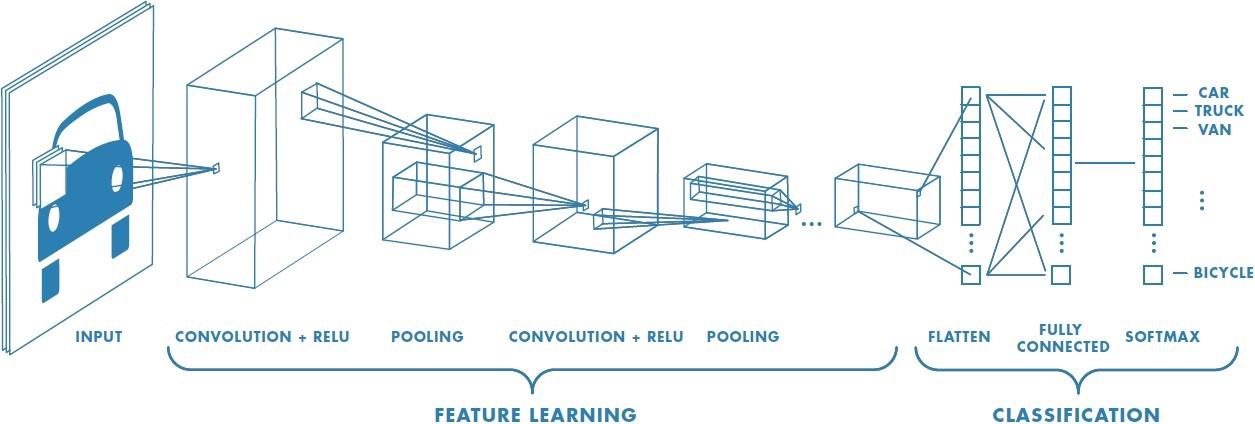
\includegraphics[height = 0.36 \linewidth]{cnn_architecture.jpeg}


    \textbf{Figure 4: CNN architecture }\cite{cnn_architecture}

\end{center}

The architecture of the neural network we used is as follows:


\begin{itemize}

    \item A rescaling layer to bring the pixel values in the interval [0, 1].

    \item 04 series of convolution layer followed by a max pooling layer.

    \item A flatten layer.

    \item Then follow a dense layer for the classification
    
    \item And finally another dense layer for the output.

\end{itemize}

\begin{center}

    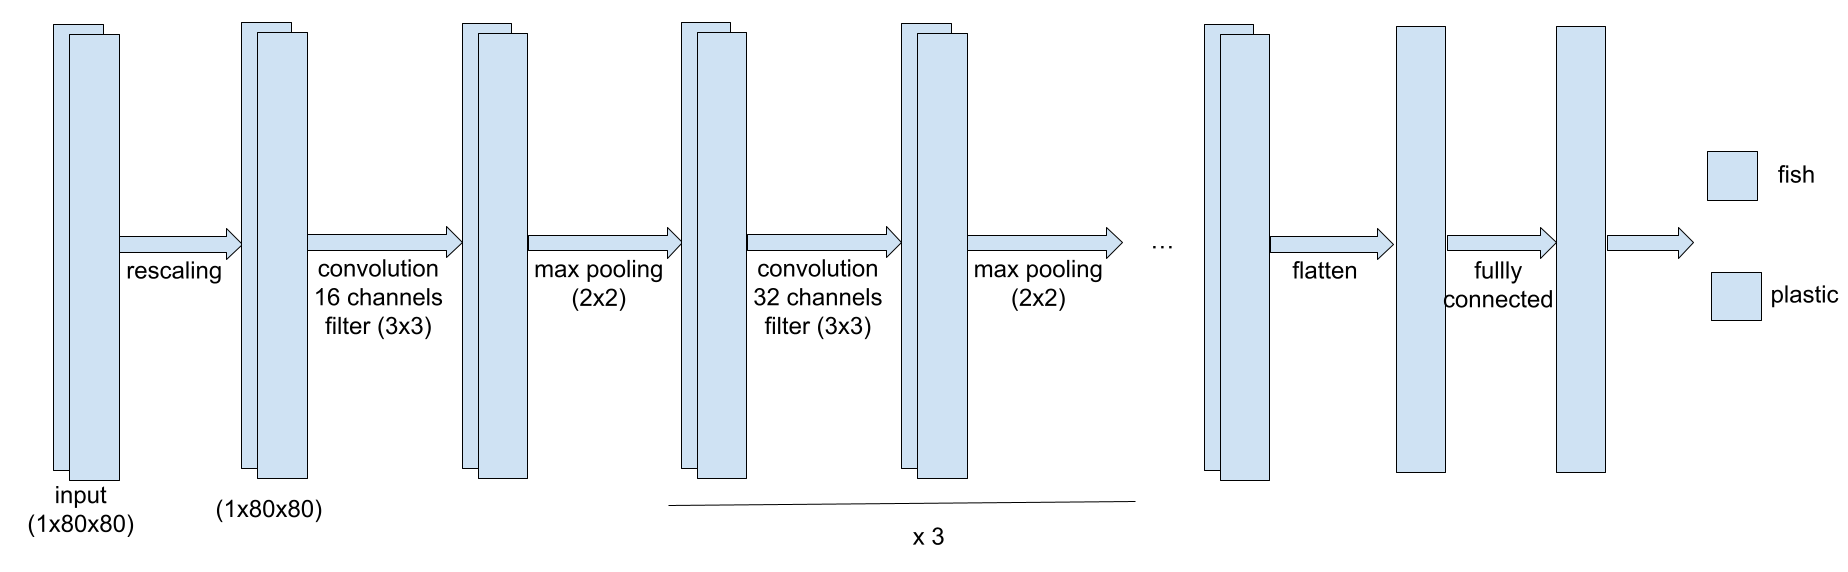
\includegraphics[height = 0.36 \linewidth]{our_nn_architecture.png}


    \textbf{Figure 5: Our Neural Network architecture }

\end{center}

\subsection{Training and testing}

After modeling our neural network, we used the tensorflow framework to implement it. And now it is the step of training and testing.

This is where performance of the algorithm, quality of data, and required output all appears out. From the huge dataset, collected 80\% of the data was used for training and 20\% for the test. Training is the process of making the machine to learn and giving it the capability to make further classifications based on the training it took. Whereas testing means already having a predefined data set with output also previously labelled and the model is tested whether it is working properly or not and is giving the right class or not. If maximum number of classificatios are right then model will have a good accuracy percentage and is reliable to continue with otherwise better to change the parameters of the model. Also, further new set of inputs and the classifications made by the model will be keep on adding to the dataset, which makes dataset more powerful and accurate. 

We have trained our model on 30 epochs with 8 steps per epochs.

\subsection{Result}

Since we used a balanced dataset, we considered it relevant to use accuracy as a performance measure for our model.

After training and testing steps, the result was pretty interesting because the model has reached 98\% of accuracy on testing.

\subsubsection{Prototype}

We have integrated our final model in a web application using Flask. we have included in the submission folder the source code of this application (in the app folder). You will find in this app folder a file "deployment\_guide.pdf" which explains how to deploy the application locally in order to test it.

After following this guide and deploying the application, below is the user guide of the application.

\begin{enumerate}

    \item Get to the test section

    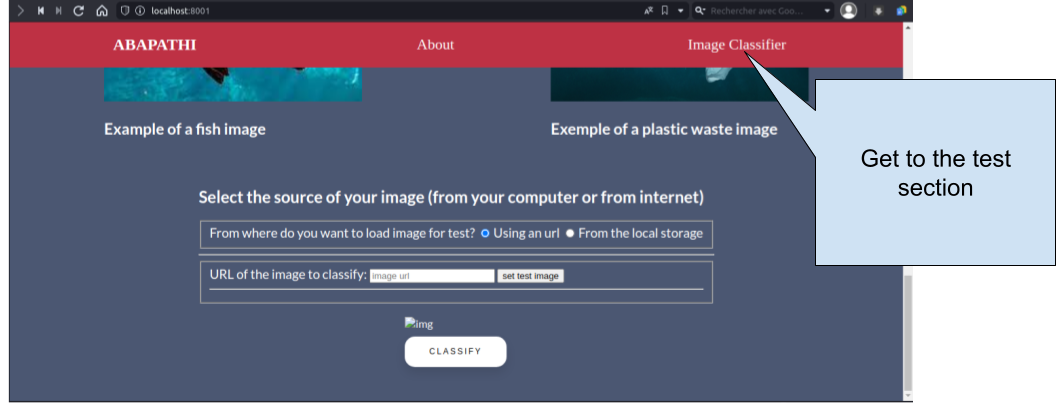
\includegraphics[height = 0.40 \linewidth]{ill_1.png}

    \item Select the image source

    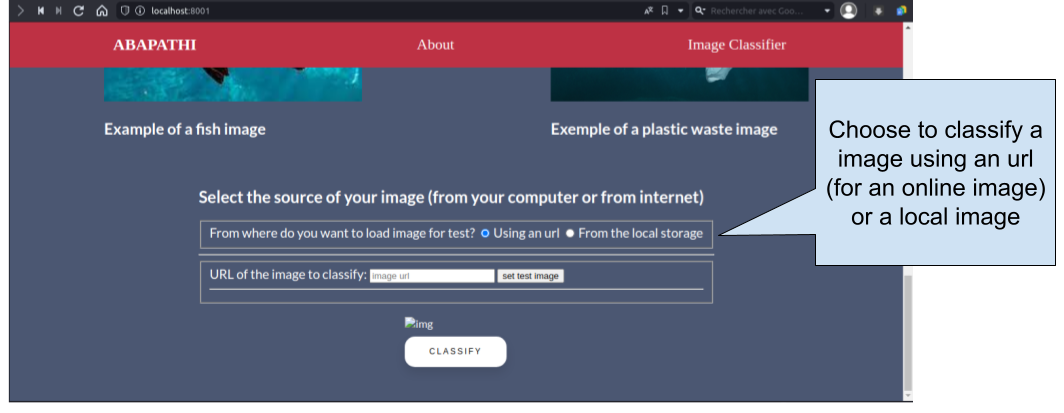
\includegraphics[height = 0.40 \linewidth]{ill_2.png}

    \item If you choosed to classify an image from the internet, go in your browser and copy the image's  address and paste it in the form.

    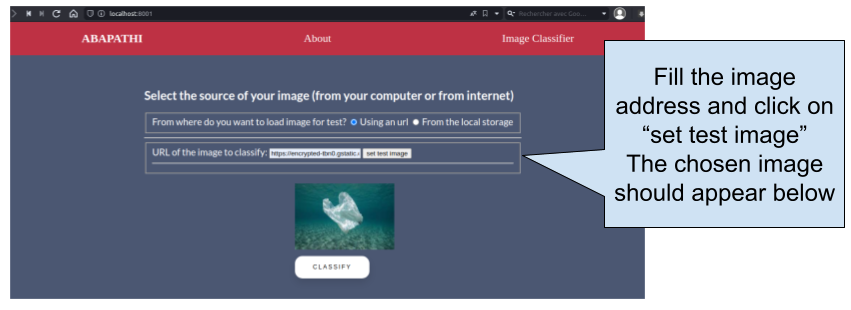
\includegraphics[height = 0.42 \linewidth]{ill_3.png}

    Ohterwise, if you choosed to classify a local image, you have to put your image in the client\_app/static/img folder, and set the image name with it's extension in the form.

    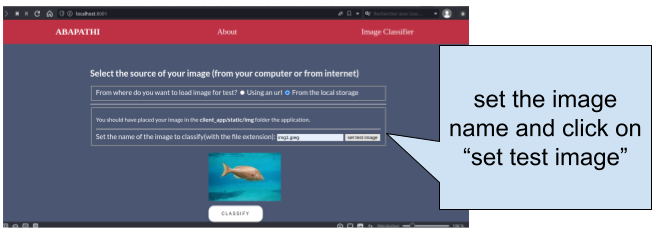
\includegraphics[height = 0.40 \linewidth]{ill_4.png}

    \item Then hit the classify button to classify the image. You will then see the result appear below the image.

    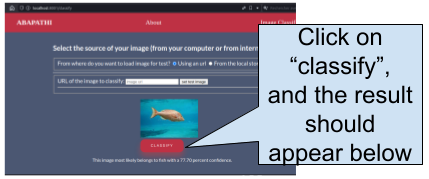
\includegraphics[height = 0.45 \linewidth]{ill_5.png}


\end{enumerate}

\section{Conclusion and future work}

In conclusion, this paper presents fish vs plastic classifier, for images taken in ocean waters. To achieve this result, we walked through a clear methodology that includes many steps (definition of the problem, data collection, data preprocessing, Deep Learning algorithm, training, testing and results).

Currently, our model works well only for fish with a specific shape like those presented on the dataset image examples. For the model to be usable it must be able to distinguish between plastics and marine animals in general, not just fish with a particular shape. To achieve this goal, it is necessary to have a large number of images of different marine species. This would greatly help to improve the performance of the model and make it usable in the real world. This is therefore a future perspective for the improvement and finalization of the model.

\renewcommand{\bibname}{References}

\begin{thebibliography}{5}
    \bibitem{razer_bot} \url{https://gamerant.com/razer-robot-cleans-trash-ocean/}

    \bibitem{fish_detection} \url{https://www.hindawi.com/journals/acisc/2020/3738108/#results-and-discussion}

    \bibitem{plastic_detection} \url{https://towardsdatascience.com/identifying-and-removing-marine-plastic-a-deep-learning-approach-6ad5e41bec41}

    \bibitem{UNEP} \url{https://www.unep.org/news-and-stories/story/tourism-pandemic-world-tackling-plastic-pollution}

    \bibitem{kaggle_fish_1} \url{https://www.kaggle.com/datasets/sripaadsrinivasan/fish-species-image-data}

    \bibitem{kaggle_fish_2} \url{https://www.kaggle.com/datasets/hiyaro/parrotfish}

    \bibitem{drive_plastic} \url{https://drive.google.com/drive/folders/1fsS_u2QpbRGynYkP6-D6cfvq8r0hpjXI}

    \bibitem{cnn_architecture} \url{https://towardsdatascience.com/a-comprehensive-guide-to-convolutional-neural-networks-the-eli5-way-3bd2b1164a53}

\end{thebibliography}

\end{document}